\documentclass[fontsize=12pt]{scrartcl}
\usepackage[ngerman]{babel}
\usepackage[utf8]{inputenc}
%\usepackage[latin1]{inputenc}
\usepackage{amsmath}
\usepackage{amstext}
\usepackage{amssymb}
\usepackage{stmaryrd}
\usepackage{verbatim}
\usepackage{mathrsfs}
\usepackage{extarrows}
\usepackage[arrow, matrix, curve]{xy}
\usepackage[centering,includeheadfoot,margin=2cm]{geometry}
\usepackage{gensymb}
\usepackage{graphicx}
\usepackage{framed}
\usepackage{xcolor}
\usepackage{float}
\usepackage{graphicx} 
\usepackage{sidecap}
\usepackage{blindtext,wrapfig}
\usepackage{epstopdf}
\usepackage{import}
\usepackage{fancyhdr}
\usepackage{fancybox}
\usepackage{graphicx}
\usepackage{caption}
\usepackage{subcaption}
\DeclareGraphicsRule{.tif}{png}{.png}{`convert #1 `basename #1 .tif`.png} 
\usepackage{fancyhdr}
\usepackage{graphicx}
\pagestyle{fancy}
\fancyhf{}
\fancyhead[R]{Physiklaisches Praktikum 1}
\fancyhead[L]{Florentin Genth, Gentian Rrafshi}
\fancyfoot[R]{Seite \thepage}
\fancyfoot[L]{\today}

\begin{document}

\begin{minipage}{\textwidth}
\begin{center}\large
\title{\textbf{Versuch O43d: Polarisation durch ein optisch aktives Medium} \\
		Assistent: Jonathan Luft \\
		Datum: 22.04.2015}

\author{bearbeitet von\\
		Gruppe 3-031: \\
		Florentin Genth Matrnr. 2952486 \\
		Gentian Rrafshi Matrnr. 2721617 }
\date{\today}

\maketitle

\end{center}
\end{minipage}

\newpage

\tableofcontents

\newpage
\noindent

\section{ Versuchsziel}

In diesem Versuch werden die Polarisationseigenschaften optisch aktiver Stoffe untersucht. Es werden ein Milchzuckerlösung und die Polarisationsfilter einer 
3D-Brille untersucht.

\section{ Grundlagen}

Grundlage dieses Versuchs ist die Polarisation. Diese beschreibt bei einer Transversalwelle, wie zum Beispiel Licht, die Richtung ihrer Schwingung. 
Es gibt verschieden Arten von Polarisationen, so ist Licht linear polarisiertes genau dann, wenn der Feldstärkevektor \emph{\textbf{E}} konstant in einer 
Richtung und einer Ebene schwingt. Eine weitere Art ist elliptisch polarisiertes Licht, welche als Überlagerung von zwei linear polarisierten Wellen angesehen 
werden, bei der die Polarisationsebenen senkrecht aufeinander gegeneinander phasenverschoben stehen. Ein Spezialfall von elliptischer Polarisation ist zirkulär 
polarisiertes Licht, dort ist die Phasenverschiebung genau $\frac{\pi}{2}$ und die Amplituden sind identisch. Zu guter Letzt gibt es noch teilweise polarisiertes 
Licht, welches Auftritt, wenn eine Schwingungsrichtung bevorzugt wird.\\
~\\
Das $\lambda/4$-Plättchen ist ein besonderes Bauteil, welches die Polarisation von linear polarisiertem Licht in zirkulär verwandelt und umgekehrt.\\
~\\
Für die Herstellung von polarisiertem Licht gibt es verschiedene Möglichkeiten:\\
~\\
\textbf{Polarisation durch Doppelbrechung:} \\
In bestimmten  nicht regulären Kristallen, wie zum Beispiel Quarzkristallen, werden verschiedene Polarisationsrichtungen unterschiedlich stark gebrochen.
Dabei unterscheidet man zwischen \glqq ordentlichen \grqq und \glqq außerordentlichen \grqq Strahlen. 
Wird ein Strahl bei senkrechtem Lichteinfall nicht gebrochen, so ist der Strahl ordentlich. Wird Strahl bei senkrechtem Lichteinfall gebrochen, so ist dieser außerordentlich. \\
~\\
\textbf{Polarisation durch Dichroismus:} \\
Manche Kristalle absorbieren nur bestimmte Polarisationsrichtungen. Bei Lichteinfall wird also nur eine bestimmte Polarisation absorbiert. Die austretenden 
Strahlen sind dann immer linear polarisiert.\\
~\\
\textbf{Polarisation durch Reflexion:} \\
Fällt zirkulär polarisiertes Licht auf eine Glasfläche, so wird dieser nicht reflektiert. Unter dem Brewsterwinkel und einem Brechungsindex wird das reflektierte 
Licht von natürlichen Licht vollständig linear polarisiert werden, wohingegen der gebrochene Strahl teilweise polarisiert ist.\\
~\\
Bestimmte Stoffe haben die besondere Eigenschaft, dass wenn man linear polarisiertes Licht auf diesen Stoff trifft, dreht sich die Polarisationsebene des 
Lichtes beim Durchgang. Solche Stoffe heißen {\textbf{optisch aktive Stoffe}}.$^{\cite{1}}$
\newpage


\section{ Versuchsaufbau und Versuchsablauf}

\begin{figure}[h]
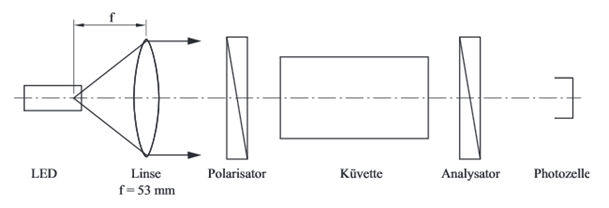
\includegraphics[scale=1]{Graphik/Versuchsaufbau}
\caption{Versuchsaufbau$^{\cite{A}}$}
\end{figure}
\subsection{Verwendete Geräte:}

\begin{itemize}
\item[•] Rote und grüne  LED
\item[•] Linse (Brennweite: 53\,mm)
\item[•] Polarisationsfilter als Polarisator und Analysator
\item[•] Küvette mit Milchzuckerlösung (Länge =1.47\,dm; Konzentration: 200\,g/Liter)
\item[•] Photozelle mit Multimeter
\item[•] 3D-Brillen
\item[•] Metallischen und weißen Schirm
\end{itemize}

\subsection{Vorbereitung:}

Der Versuch wird  der Skizze entsprechend aufgebaut. Zuerst wird die grüne LED verwendet. Diese wird in den Brennpunkt der Linse  gelegt, um parallele 
Lichtstrahlen zu erzeugen, und dabei so eingestellt, dass der Strahl mittig auf die Photozelle trifft. Diese ist an ein Multimeter angeschlossen, das den 
Kurzschlussstrom der Zelle misst, welcher zu der einfallenden Lichtintensität proportional ist, solange der Strom 100\,$\mu$A nicht überschreitet Dann 
werden Polarisator und Analysator so eingestellt, dass  das Licht mit maximaler Intensität auf die Photozelle trifft.  Sie sollten beide in der 0$^\circ$-Stellung 
sein. Diese Anordnung soll in den folgenden Versuchen nicht verändert werden. Die Messung erfolgt, indem man den Analysator in 10$^{\circ}$-Schritten 
einmal vollständig von 0$^\circ$ bis 360$^\circ$ dreht. Die resultierende Lichtintensität wird dem Multimeter als Kurzschlussstrom entnommen.

\subsection{Versuch 1: Bestimmung des Drehvermögens von Lactose}
Zuerst wird die Intensitätsänderung des grünen Lichts ohne Milchzuckerlösung gemessen, dann setzt man die Küvette mit der Milchzuckerlösung zwischen 
Polarisator und wiederholt die Messprozedur.  Anschließend ersetzt man die grüne LED durch die rote und wiederholt den Versuch. Man erhält insgesamt 4 
Messreihen.

\subsection{Versuch 2: Untersuchung einer 3D-Brille}

In diesem Versuch wird dieKüvette mit der Milchzuckerlösung durch die 3D-Brillen-Halterung ersetzt. Für den ersten Teil des Versuchs werden Analysator 
und Photozelle mit Multimeter nicht benötigt, für den zweiten Teil jedoch schon.

\subsubsection{Voruntersuchung}
Als Voruntersuchung wird die Brille betrachtet und festgestellt, auf welche Seite sich der Polarisationsfilter befindet, d.h. auf welcher Seite linear polarisiertes 
Licht austritt. Dafür betrachtet man zuerst die Vorderseite, dann die Rückseiteder Brille mit einem Polarisationsfilter und überprüft, ob die Rotation der Brille 
die transmittierte Intensität verändert, was bei linear polarisierten Licht der Fall wäre, und notiert die Ergebnisse. Anschließend setzen zwei Menschen jeweils 
eine Brille auf und man notiert, mit welchem Auge man welches Auge des Gegenübers sehen kann und welches Auge abgedunkelt wird.

\subsubsection{Durchführung}
Nun wird die Brille so eingespannt, dass zirkular polarisiertes Licht auf einen metallischen Schirm trifft, das in 45$^\circ$ zum Lichtstrahl orientiert ist. Zuerst 
wird grünes Licht durch das rechte \glqq Glas \grqq  der Brille gestrahlt. Man betrachtet man resultierenden Lichtfleck erst durch das linke, dann durch das 
rechte Glaseiner weiteren 3D-Brille und notiert die Ergebnisse. Anschließend überprüft man, ob die Intensität von der Ausrichtung der Brillen abhängig ist und 
notiert die Ergebnisse. Dasselbe macht man für das linke Glas der Brille.
Dann ersetzt man die grüne LED durch die rote, wiederholt den Versuch und notiert die Ergebnisse.
Als nächstes wird der der metallische Schirm durch einen weißen ersetzt und der Versuch nochmal wiederholt und die Ergebnisse notiert.
Nun wird der Schirm entfernt, sodass der Lichtstrahl wieder durch Polarisator, 3D-Brille und Analysator auf die Photozelle trifft. Man misst wie in Versuch 1 
für rotes Licht und grünes Licht jeweils in 10$^\circ$-Schritten von 0$^\circ$ bis 360$^\circ$ die Intensität des Lichts durch Rotation des Analysators und 
notiert die jeweiligen Kurzschlussströme. 
\newpage
\section{ Formeln}

\subsection{Formel für das spezifische Drehvermögen über Drehung der Polarisationsebene}

Zur Berechnung des spezifischen Drehvermögens benötigen wir die Formel:
\begin{equation}
\alpha = \frac{\Delta\varphi}{l \cdot c}
\end{equation}
\\
Wobei $\alpha$ die spezifische optische Drehung, $\Delta \varphi$ in [$^\circ$] die Winkeldifferenz der Drehung der Polarisationsebene, $l$ in [dm] die Länge der Küvette und $c$ in [g/dm$^3$] die Konzentration 
der optisch aktiven ist. \\

\subsection{Formel für das spezifische Drehvermögen über Natrium-D-Linie}
In der Auswertung werden unsere Werte mit den Literaturwerten verglichen, dazu benötigen wir folgende Formel:
\begin{equation}
\alpha(\lambda)=\alpha(589\,\text{nm})\cdot (\frac{589\,\text{nm}}{\lambda})^2
\end{equation}
Hier ist wieder $\alpha$ die spezifische optische Drehung.

\section{ Messwerte}

Die originalen Messwerte liegen in Anhang.

\newpage
\section{ Auswertung}

\subsection{Auswertung des Drehvermögens von Lactose}
Zunächst werden zur Bestimmung des Drehwinkels $\Delta\varphi$ die gemessen Stromstärken in Abhängigkeit des Winkels in als lineares Diagramm 
dargestellt. Das erste Diagramm ist die Messung ohne Küvette, das zweite mit Küvette.
\begin{figure}[H]
\vspace{-12pt}
		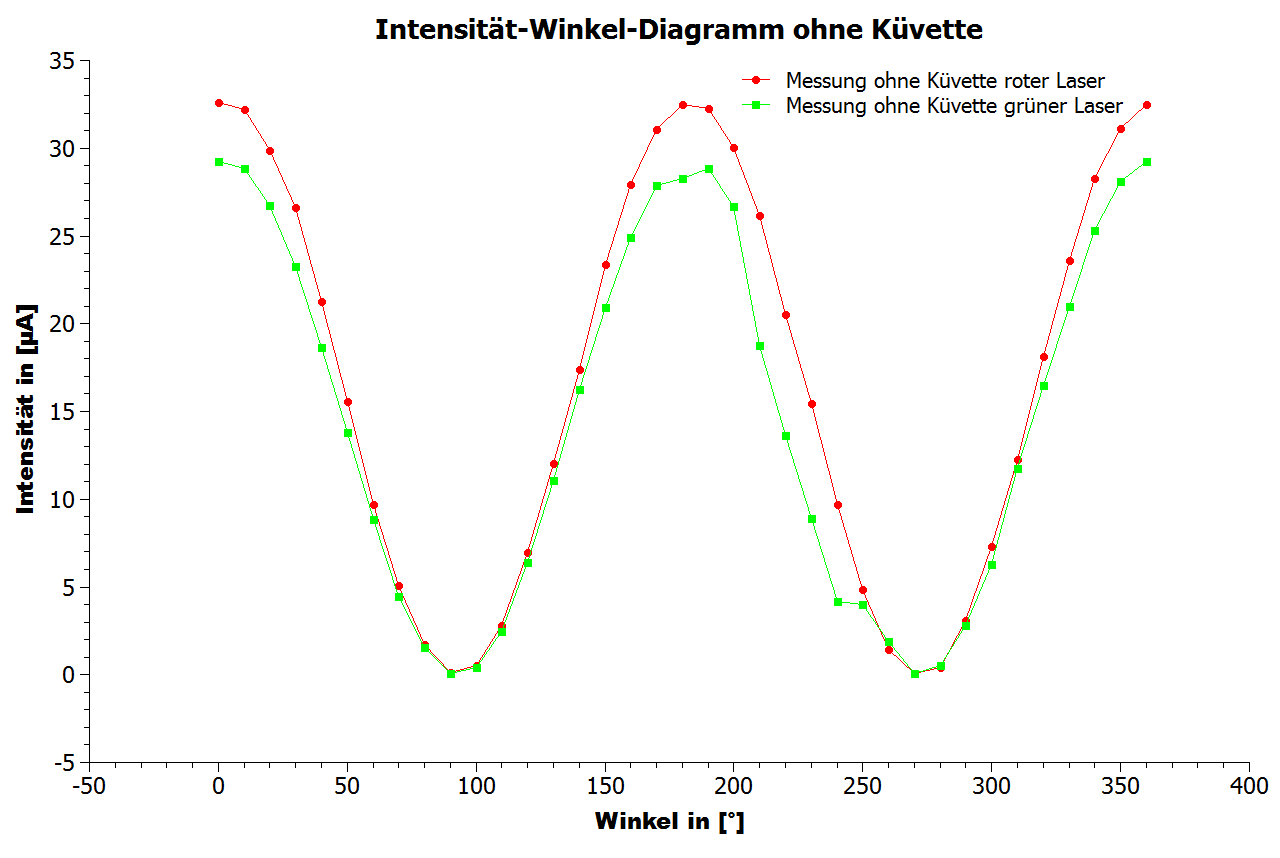
\includegraphics[scale=0.4]{Graphik/Intensitats-Winkel-Diagramm-ohne-Kuvette}
		\vspace{-15pt}
		\caption{Intensität-Winkel-Diagramm-ohne-Küvette}
\end{figure}
\begin{figure}[H]
\vspace{-17pt}
        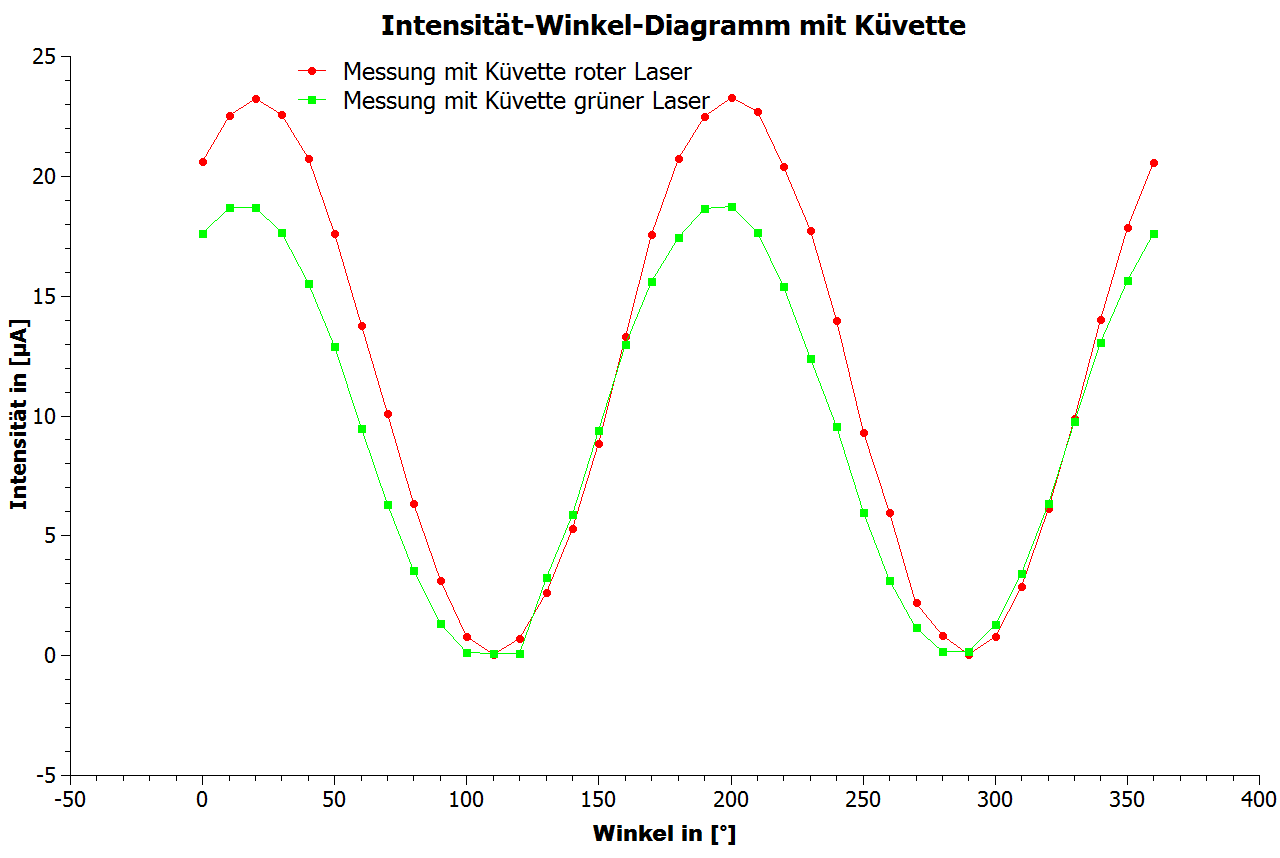
\includegraphics[scale=0.4]{Graphik/Intensitats-Winkel-Diagramm-mit-Kuvette}
        \vspace{-10pt}
		\caption{Intensität-Winkel-Diagramm-mit-Küvette}
\end{figure}
\noindent
Dann werden zur Bestimmung des Drehwinkels $\Delta\varphi$ die gemessen 
Stromstärken in einem Polar-Diagramm dargestellt. \\
~\\
Zuerst das Diagramm für die rote LED, dann grüner LED:
\begin{figure}[H]
\vspace{-12pt}
		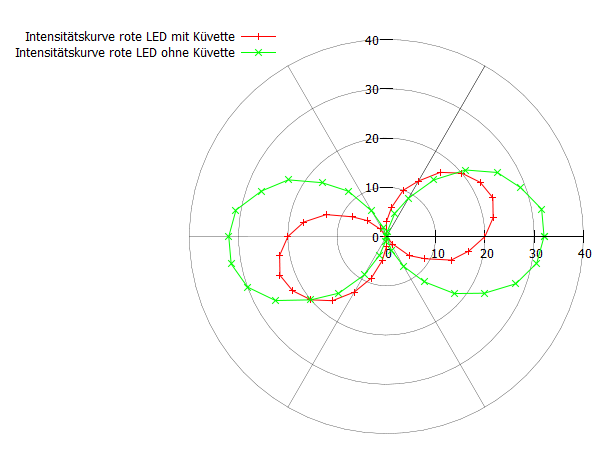
\includegraphics[scale=0.75]{Graphik/PolarroteLED}
		\vspace{-15pt}
		\caption{Intensität-Winkel-Diagramm rote LED}
\end{figure}
\begin{figure}[H]
\vspace{-17pt}
        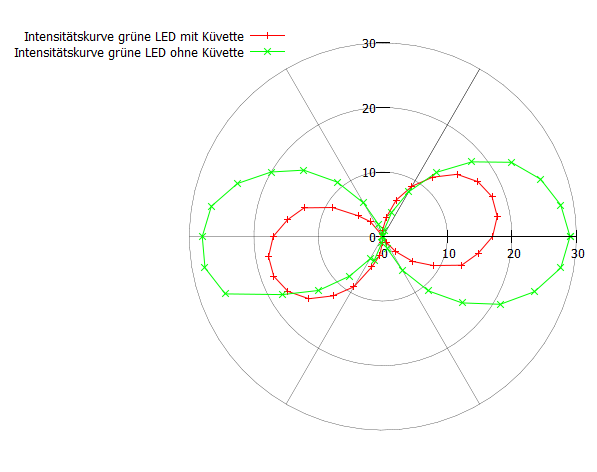
\includegraphics[scale=0.75]{Graphik/PolargruneLED}
        \vspace{-10pt}
		\caption{Intensität-Winkel-Diagramm grüne LED}
\end{figure}
\noindent
Aus diesem Diagramm kann nun $\Delta\varphi$ bestimmt werden. Das Intensität-Winkel-Diagramm-ohne-Küvette zeigt uns, dass es für den Versuch besser 
ist, Minima statt Maxima zu nehmen, da ein Maxima Fehler enthält, dazu mehr später. Die Bestimmung erfolgt, in dem man den Winkel des Minima mit der 
Küvette bestimmt (erst für rotes, dann für grünes Licht) und diesen von dem Winkel des Minima ohne Küvette abzieht, welchen man ebenfalls dem Diagramm 
entnehmen kann. 
Mit $\Delta\varphi$ und Formel 1 kann man die spezifische optische Drehung für jeweils grünes und rotes Licht berechnen. \\
~\\
Die abgelesenen Messwerte werden in folgender Tabelle dargestellt:
\begin{figure}[h]
\centering
\caption{Minima zur Bestimmung von $\Delta\varphi$}
\begin{tabular}{|l|c|c|} \hline
Minima  & bei rotem Laser  & bei grünem Laser\\ \hline
Winkel ohne Küvette [$^\circ$]  & 270  & 270 \\ \hline
Messwert [$\mu$A]& 0,06 & 0,08  \\ \hline
Winkel mit Küvette [$^\circ$] & 290  & 290 \\ \hline
Messwert [$\mu$A] & 0,05  & 0,17  \\ \hline 
Winkeldifferenz $\Delta\varphi$ [$^\circ$]& 20 & 20 \\ \hline 
\end{tabular} \\
\end{figure}
\noindent
Aus diesen Messwerten und Formel (1) lässt sich nun die spezifische Drehung bestimmen. Beispielhaft wird hier eine Rechnung für den roten Laser durchgeführt:
\begin{align*}
\alpha = \frac{\Delta\varphi}{l \cdot c} = \frac{ 20 \cdot 1000}{1,47\,\text{dm} \cdot 200\,\text{g/ml}} =  68,02721088\,\frac{ ^\circ \cdot \text{ml}}{\text{dm $\cdot$ g}}
\end{align*}
Die errechneten Ergebnisse werden in folgender Tabelle eingefügt:
\begin{figure}[h]
\centering
\caption{Rechenergebnisse für $\alpha$}
\begin{tabular}{|c|c|c|} \hline
  & bei rotem Laser  & bei grünem Laser\\ \hline
spezifischer Drehwinkel $\alpha$ [$\frac{ ^\circ \cdot \text{ml}}{\text{dm $\cdot$ g}}$]  & 68,03  & 68,03  \\ \hline
\end{tabular} \\
\end{figure}

\newpage
\noindent
Die Werte sollen mit dem Literaturwert verglichen werden. Wofür wir Formel 2 benötigen. Für $\alpha(589$\,nm) nehmen wir den Wert
$\alpha(589$\,nm) $=+53,6\,[\frac{ ^\circ \cdot \text{ml}}{\text{dm $\cdot$ g}}$].$^{\cite{2}}$
An einem Beispiel wird hier nachgerechnet, danach werden die Werte eine die Tabelle eingetragen.
\begin{equation*}
\alpha(525\,\text{nm})=+53,6\,\frac{ ^\circ \cdot \text{ml}}{\text{dm $\cdot$ g}}\cdot (\frac{589\,\text{nm}}{525\,\text{nm}})^2=67,4647278005\,\frac{ ^\circ \cdot \text{ml}}{\text{dm $\cdot$ g}} \approx 67,46\,\frac{ ^\circ \cdot \text{ml}}{\text{dm $\cdot$ g}}
\end{equation*}
\begin{figure}[h]
\centering
\caption{Rechenergebnisse für $\alpha$}
\begin{tabular}{|l|c|c|} \hline
  & bei rotem Laser  & bei grünem Laser\\ \hline
spezifischer Drehwinkel $\alpha$ mit Formel (1) [$\frac{ ^\circ \cdot \text{ml}}{\text{dm $\cdot$ g}}$]  & 68,03  & 68,03  \\ \hline
spezifischer Drehwinkel $\alpha$ mit Formel (2) [$\frac{ ^\circ \cdot \text{ml}}{\text{dm $\cdot$ g}}$]  & 46,12  & 67,46  \\ \hline
\end{tabular} \\
\end{figure}
\newpage
\noindent
\subsection{Auswertung des Versuchs über die 3D-Brille }

\subsubsection{Voruntersuchung:}
Durch die oben beschriebene Vorgehensweise kann man feststellen, dass sich der Polarisationsfilter sich auf der Rückseite der Brille, also auf der dem Gesicht 
des Trägers zugewandten Seite befindet und sich auf der anderen Seite ein $\lambda/4$-Plättchen befindet. Der Vorteil dieser Anordnung ist, dass die 3D-
Brille unabhängig der Ausrichtung der Brille funktioniert, so dass der Träger sein Kopf nicht zu jeder Zeit senkrecht halten muss. \\
~\\
Zudem kann man feststellen, dass man mit dem linken Auge durch die Brille das linke Auge des Gegenübers sehen kann. Dies ist der Fall, weil beide Brillen denselben Aufbau haben und  somit die Drehrichtung des zirkular polarisierten Lichts für jeweils das linke Augen und das rechte Auge gleich ist.

\subsubsection{Hauptversuch:}
Bei dem metallischen Schirm wurde beobachtet, dass man das mit dem rechten Glas produzierte zirkular polarisierte grüne Licht nach Reflektion am Schirm 
durch das linke Glas betrachtet gut sehen konnte, es durch das rechte Glas hingegen deutlich abgeschwächt wurde. Rotiert man die Brille, so stellt man eine 
minimale Abschwächung fest. Das grüne Licht wird also annähernd zirkular polarisiert. Durch die Reflektion wurde aber die Drehrichtung des zirkular 
polarisierten. Bei der roten LED passiert dasselbe, es kommt jedoch zu einer deutlicheren Abschwächung bei Rotation, woran man erkennen kann, dass das 
rote Licht elliptisch polarisiert wird. Dies liegt daran, dass bei einem $\lambda/4$-Plättchen die Dicke entscheidend ist. Das $\lambda/4$-Plättchen der 3D-
Brille ist so dick, dass grünes linear polarisiertes Licht zu zirkular polarisierten wir und umgekehrt. Fällt nun rotes Licht durch das Plättchen, so wird zirkular 
polarisiertes Licht nicht vollständig linear, sondern elliptisch, ebenso wird lineares Licht nicht vollständig zirkular. \\
~\\
Bei dem weißen Schirm stellt man fest, dass man immer einen Lichtfleck auf dem Schirm sieht, unabhängig von Lichtfarbe und durch welches Glas man sieht. 
Alles einfallende Licht wird bei der Reflektion also unpolarisiert. Nun wird mit Analysator und Photozelle die oben schon beobachtete Intensitätsänderung bei 
Rotation der Brille gemessen. Es werden dieselben Beobachtungen gemacht: grünes Licht wird annähernd zirkular polarisiert und rotes Licht elliptisch.\\
~\\
Anhand dieses Versuchs kann man nun Rückschlüsse auf die Funktionsweise einer 3D-Brille ziehen:\\
Im Kino wird das „linke“ Bild in eine Richtung zirkular polarisiert und das „rechte“ Bild in die andere Richtung. Diese werden nun auf eine auf eine metallische 
Leinwand projiziert, sodass sie zirkular reflektiert werden (wobei die Drehrichtung umgekehrt wird). Nun sorgen das $\lambda/4$-Plättchen und der 
Polarisationsfilter der Brille dafür, dass nur die Lichtstrahlen das Auge erreichen, die annähernd zirkular polarisiert sind und die richtige Drehrichtung besitzen. 
Dadurch sieht man mit jedem Auge ein anderes Bild, wodurch der 3D-Effekt zustande kommt.\\
~\\
Zu guter Letzt werden unsere Messwerte in ein Polardiagramm eingezeichnet:
\begin{figure}[H]
\vspace{-17pt}
        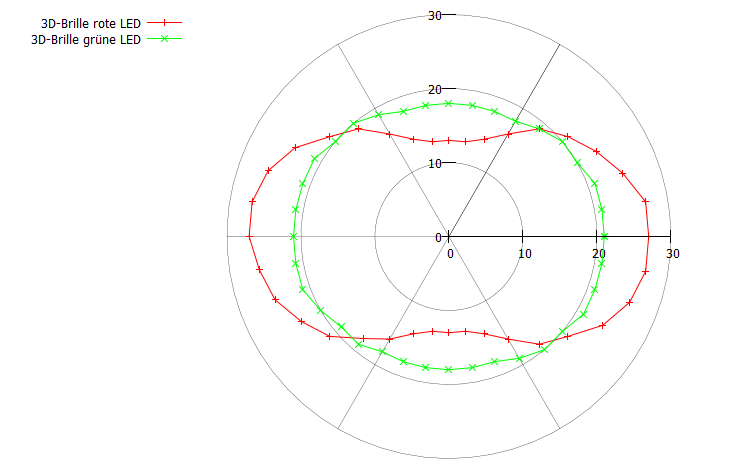
\includegraphics[scale=0.75]{Graphik/3D}
        \vspace{-10pt}
		\caption{Intensität-Winkel-Diagramm der 3D-Brille}
\end{figure}
\noindent
\newpage
\section{Fehlerrechnung}

\subsection{Fehlerquellen}

Wie schon in der Auswertung genannt, ist ein Fehler in dem Intensität-Winkel-Diagramm-ohne-Küvette zu sehen, bei 170$^\circ$-200$\circ$.
Dieser Fehler erklärt sich unserer Meinung nach dadurch, dass zu dem Augenblick der Messung die 1. Gruppe fertig war und beim verlassen des Versuchsraum die Tür länger auf war und dadurch  der Raum auch heller war. \\
~\\
Eine weitere Quelle war das Messgeräte, mit der wir die Intensität bestimmten. Oft gab es Schwankungen im $\pm 2\,\mu$A. Bemerkten wir dies, warteten wir ein paar Sekunden. Dann hatte sich das Gerät eingependelt und  nahmen den eingependelten Wert als Messwert. 

\subsection{Fehlerrechnung spezifischer Drehwinkel}

Bei der Winkelmessung nehmen wir einen Fehler von $1^\circ$ an, da der Winkelmesser in $1^\circ$-Schritten verlief. Diesen Fehler nennen wir aus optischen Gründen nicht $\Delta (\Delta \varphi)$, sondern $\Delta\varphi_{\text{Fehler}}$.\\
~\\
Für den Fehler von $\Delta \alpha$ ergibt sich dann mit Hilfe von Formel 1:
\begin{align*}
\Delta \alpha &= \vert \Delta\varphi_{\text{Fehler}} \cdot \frac{\partial}{\partial~\Delta\varphi} \frac{\Delta\varphi}{l \cdot c} \vert \\
&= \vert  \frac{\Delta\varphi_{\text{Fehler}}}{l \cdot c} \vert = \vert \frac{ 1 \cdot 1000}{1,47\,\text{dm} \cdot 200\,\text{g/ml} }\vert  \\
&= 3,4013605442176871\,\frac{ ^\circ \cdot \text{ml}}{\text{dm $\cdot$ g}}  \approx 3,40\,\frac{ ^\circ \cdot \text{ml}}{\text{dm $\cdot$ g}}
\end{align*}
\noindent 
Zuletzt noch eine Tabelle mit unseren Werten für $\alpha$ samt Fehler $\Delta\alpha$ :
\begin{figure}[h]
\centering
\caption{Rechenergebnisse und Fehler für $\alpha$}
\begin{tabular}{|l|c|c|} \hline
  & bei rotem Laser  & bei grünem Laser\\ \hline
spezifischer Drehwinkel $\alpha$ [$\frac{ ^\circ \cdot \text{ml}}{\text{dm $\cdot$ g}}$]  & 68,03  & 68,03  \\ \hline
Fehler spezifischer Drehwinkel  $\Delta \alpha$ [$\frac{ ^\circ \cdot \text{ml}}{\text{dm $\cdot$ g}}$]  & $\pm$ 3,40  & $\pm$ 3,40  \\ \hline
\end{tabular} \\
\end{figure}
\newpage
\noindent

\section{Zusammenfassung}

Im ersten Versuchsteil sollten wir den spezifischen Drehwinkel $\alpha$ für roten und grünen Laser bestimmen und mit dem Hilfe von Formel 2 verglichen werden. Unser Ergebnisse werden in einer Tabelle zusammengefasst:
\begin{figure}[h]
\centering
\caption{Zusammenfassung al unserer Messergebnisse}
\begin{tabular}{|l|c|c|} \hline
 & bei rotem Laser  & bei grünem Laser\\ \hline
Winkel Minima ohne Küvette [$^\circ$]  & 270  & 270 \\ \hline
Messwert [$\mu$A]& 0,06 & 0,08  \\ \hline
Winkel Minima mit Küvette [$^\circ$] & 290  & 290 \\ \hline
Messwert [$\mu$A] & 0,05  & 0,17  \\ \hline 
Winkeldifferenz $\Delta\varphi$ [$^\circ$]& 20 & 20 \\ \hline 
spezifischer Drehwinkel $\alpha$ [$\frac{ ^\circ \cdot \text{ml}}{\text{dm $\cdot$ g}}$]  & 68,03  & 68,03  \\ \hline
Fehler spezifischer Drehwinkel  $\Delta \alpha$ [$\frac{ ^\circ \cdot \text{ml}}{\text{dm $\cdot$ g}}$]  & $\pm$ 3,40  & $\pm$ 3,40  \\ \hline
spezifischer Drehwinkel $\alpha$ mit Formel (2) [$\frac{ ^\circ \cdot \text{ml}}{\text{dm $\cdot$ g}}$]  & 46,12  & 67,46  \\ \hline
\end{tabular} \\
\end{figure}
\noindent
Beim grünen Laser sind wir sehr nah an dem mit Formel 2 errechneten Literaturwert. Wir liegen damit sogar in der Fehlertoleranz. Dies gilt allerdings nicht für 
den roten Laser, wo unsere Abweichung sehr groß ($\approx 32,21\,\%$).  \\
~\\
Bei der 3D-Brille fanden wir heraus, dass auf der Außenseite der 3D-Brille sich das $\lambda/4$-Plättchen und auf der Innenseite der Polarisationfilter 
befindet. Auch haben wir herausgefunden, dass das rote Licht in der 3D-Brille elliptisch polarisiert und das grüne Licht zirkulär polarisiert wird, dass liegt am 
$\lambda/4$-Plättchen der 3D-Brille. Dieses ist so dick, dass grünes linear polarisiertes Licht zu zirkular polarisierten wir und umgekehrt. Fällt nun rotes Licht durch das Plättchen, so wird zirkular polarisiertes Licht nicht vollständig linear, sondern elliptisch, ebenso wird lineares Licht nicht vollständig zirkular.
Diese Ergebnisse erhält man beim metallischen Schirm. Beim dem weißen Schirm stellt man fest,  dass alles einfallende Licht wird bei der Reflektion  unpolarisiert bleibt. Die selben Ergebnisse erhält man durch die Verwendung des Analysators.
~\\
Die Funktionsweise der 3D-Brille erklärt sich durch diesen Versuch. So wird das „linke“ Bild in eine Richtung zirkular polarisiert und das „rechte“ Bild in die andere Richtung. Im Kino wird dies dann auf einer metallischen Leinwand projiziert. Das $\lambda/4$-Plättchen und der Polarisationsfilter der Brille
sorgen dann dafür, dass wir mit jedem Auge ein anderes Bild sehen, welches den 3D-Effekt hervorruft.
\newpage
\section{Literaturverzeichnis}

\begin{thebibliography}{xxxx}
	\bibitem[1]{1}	textit{\glqq O43 Polarisation durch ein optisch aktives Medium\grqq , in http://www3.physik.uni-stuttgart.de/studium/	
    						praktika/ap/}, \textit{ unter 	http://www3.physik.uni-stuttgart.de/studium/praktika/ap/pdf\_dateien/O43.pdf abgerufen am 28.04.2015}
   \bibitem[2]{2}   	H.-D. Belitz, W. Grosch und P. Schieberle, \textit{ Lehrbuch der Lebensmittelchemie}, Springer-Verlag, Berlin,~\textbf{2001}, S.246 				                        Tabelle 4.8
    \bibitem[A]{A}  Graphik aus \textit{\glqq O43 Polarisation durch ein optisch aktives Medium\grqq , in http://www3.physik.uni-stuttgart.de/studium/	
    							praktika/ap/}, \textit{ unter 	http://www3.physik.uni-stuttgart.de/studium/praktika/ap/pdf\_dateien/O43.pdf abgerufen am 28.04.2015}
\end{thebibliography}
\newpage

\section{Anhang}
Hier sind die original Messdaten, welche eingescannt wurden
\begin{figure}[H]
\vspace{-17pt}
        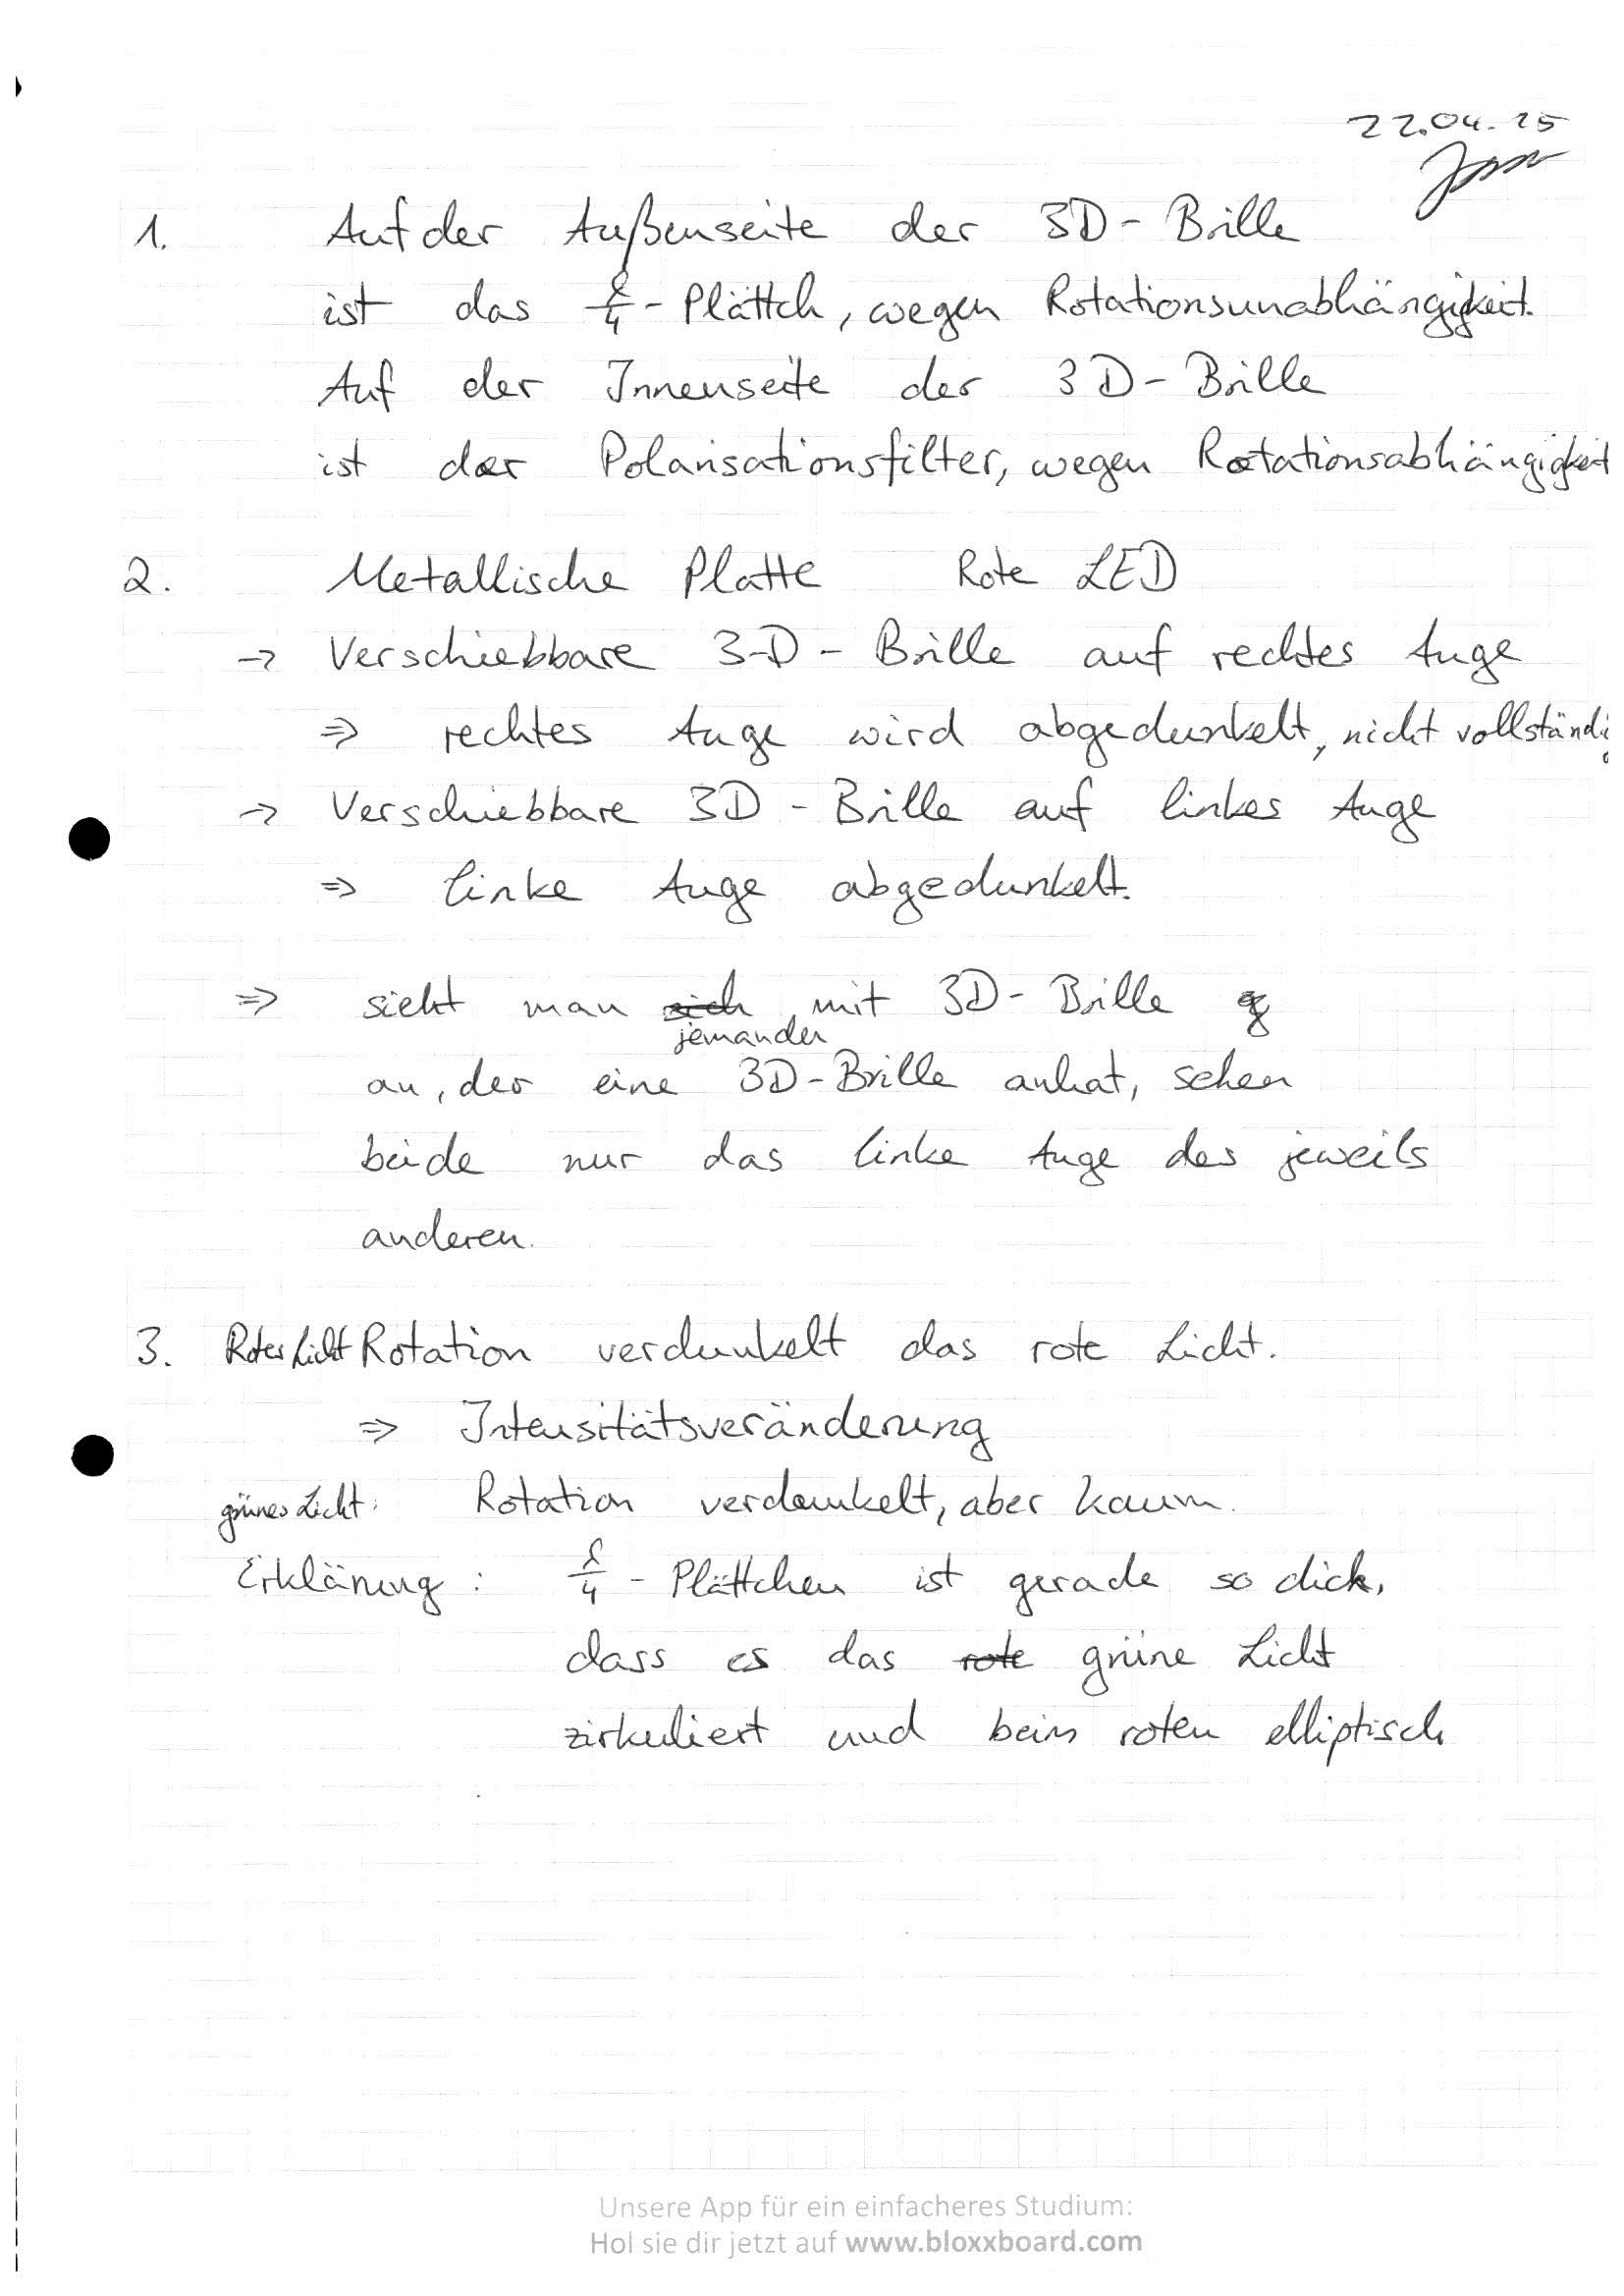
\includegraphics[scale=0.6]{Graphik/1}
        \vspace{-10pt}
\end{figure}
\begin{figure}[H]
\vspace{-17pt}
        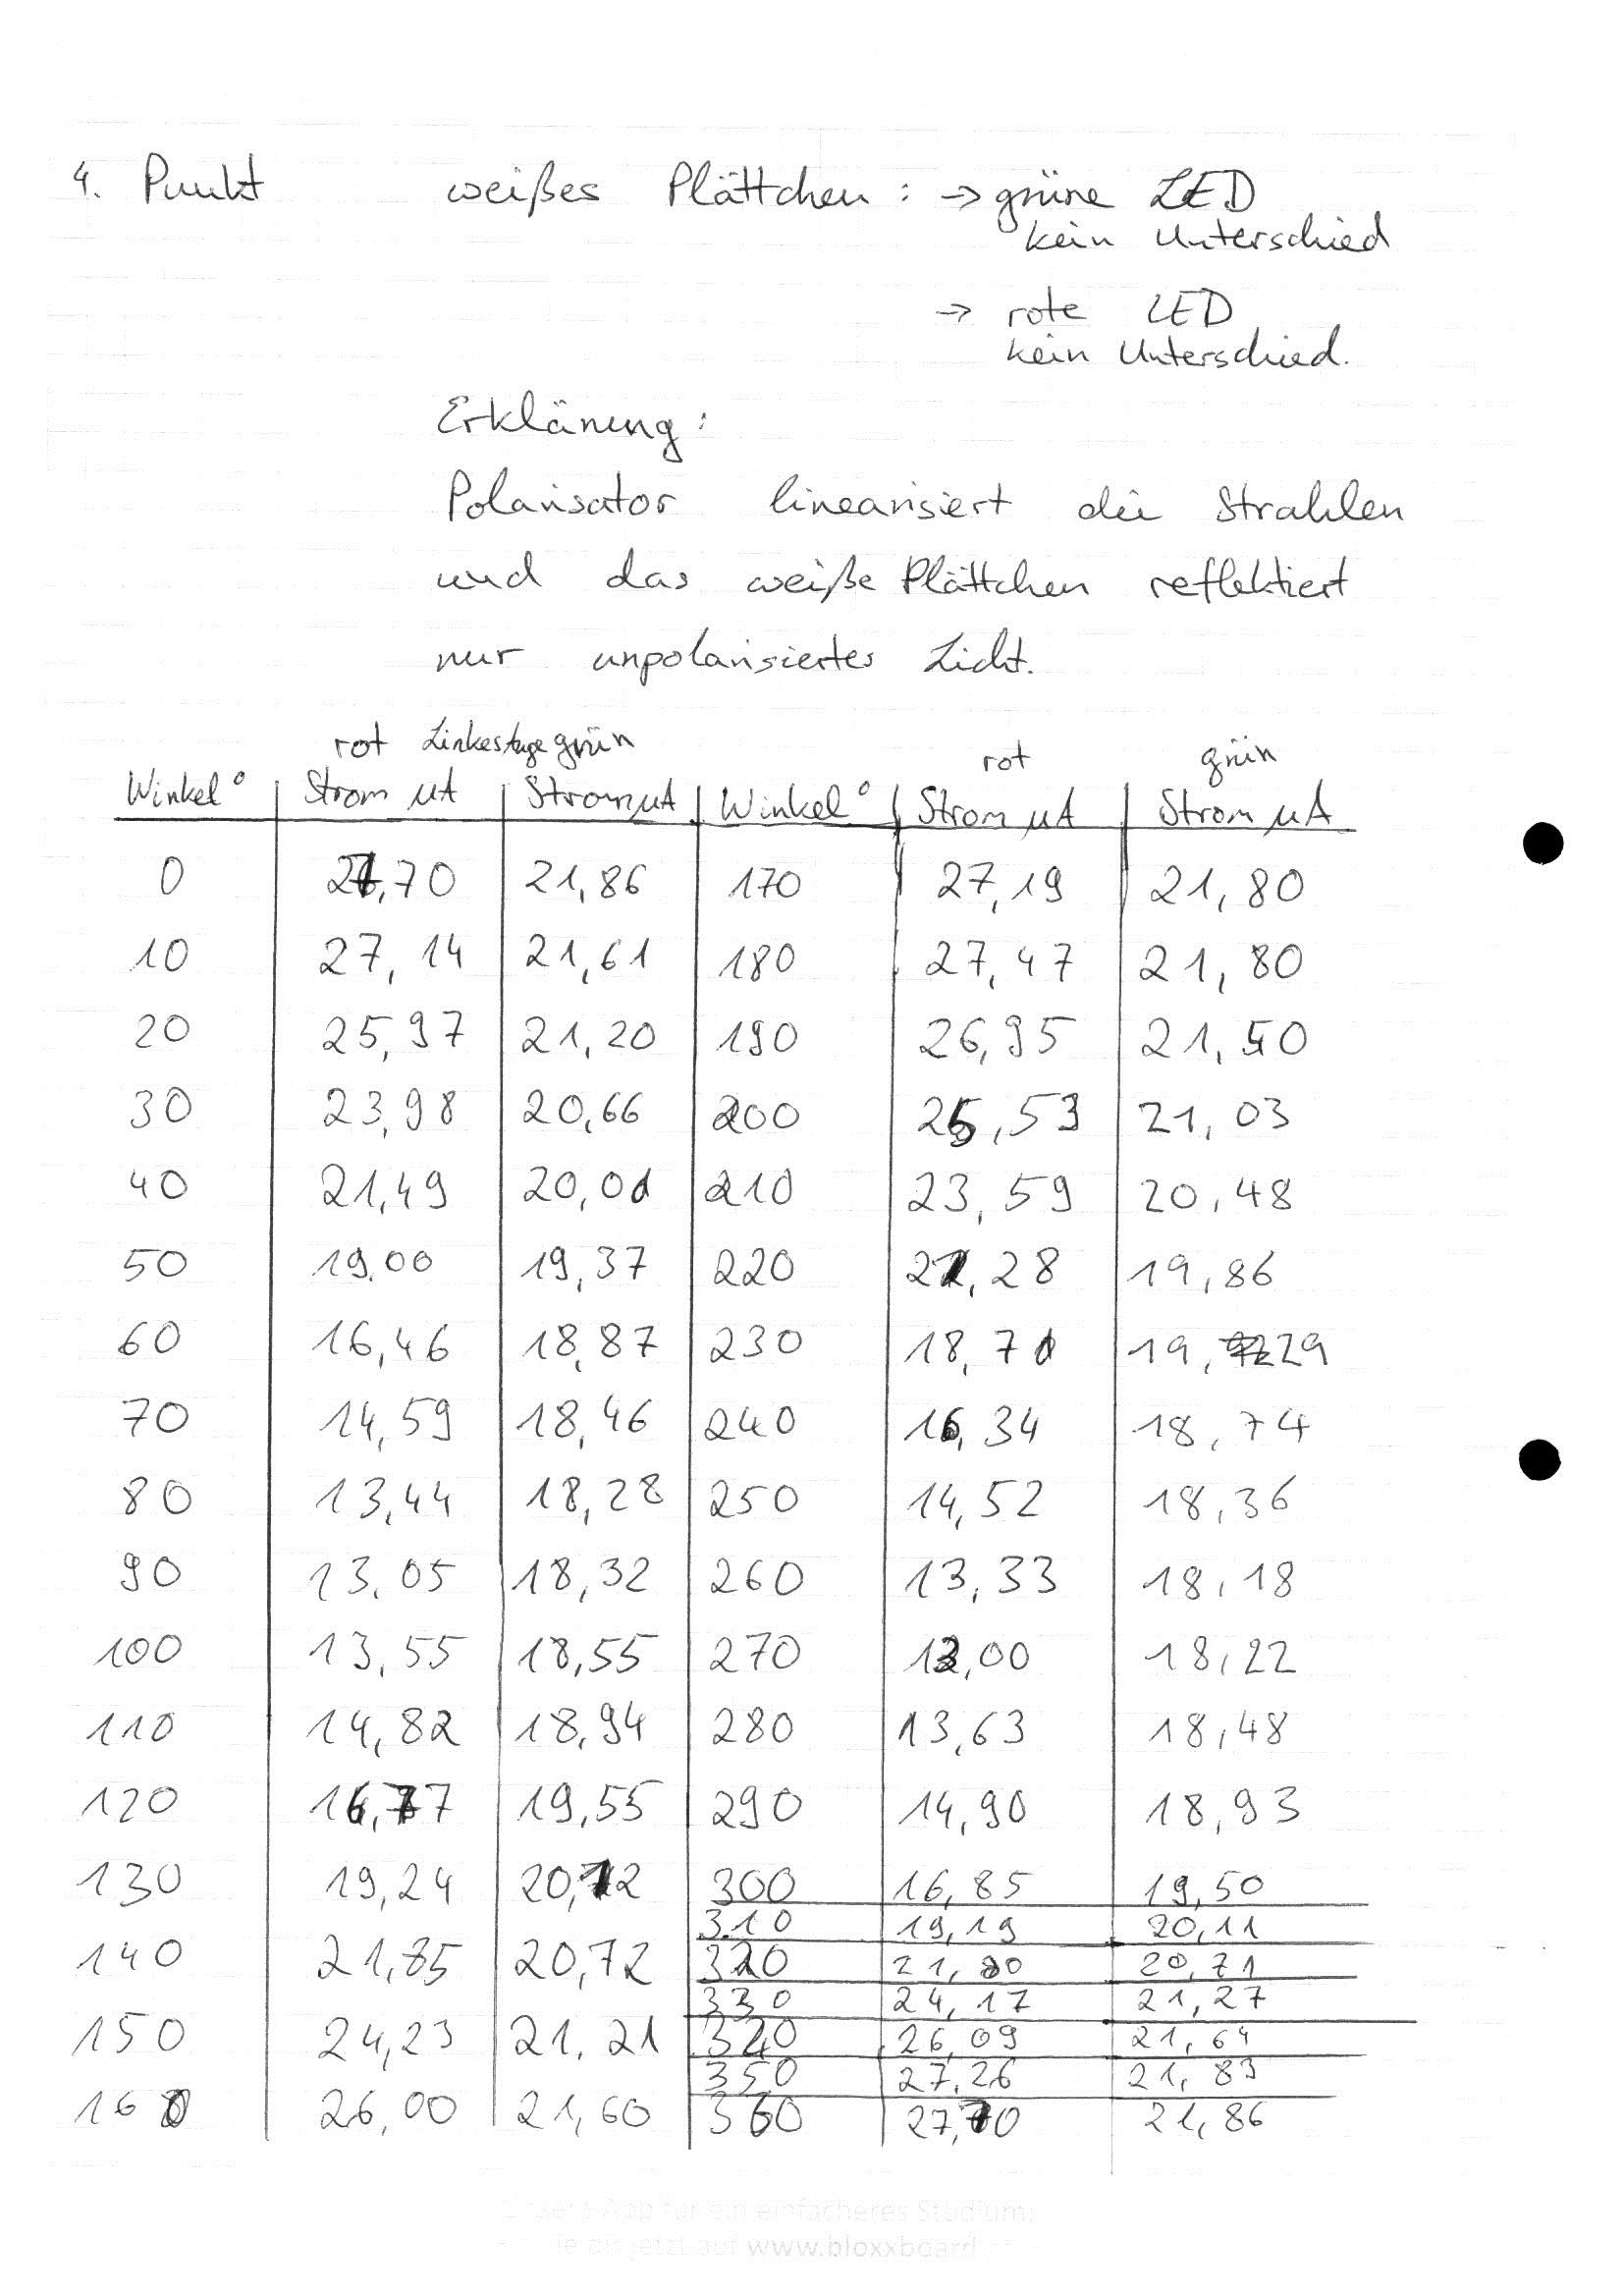
\includegraphics[scale=0.6]{Graphik/2}
        \vspace{-10pt}

\end{figure}
\begin{figure}[H]
\vspace{-17pt}
        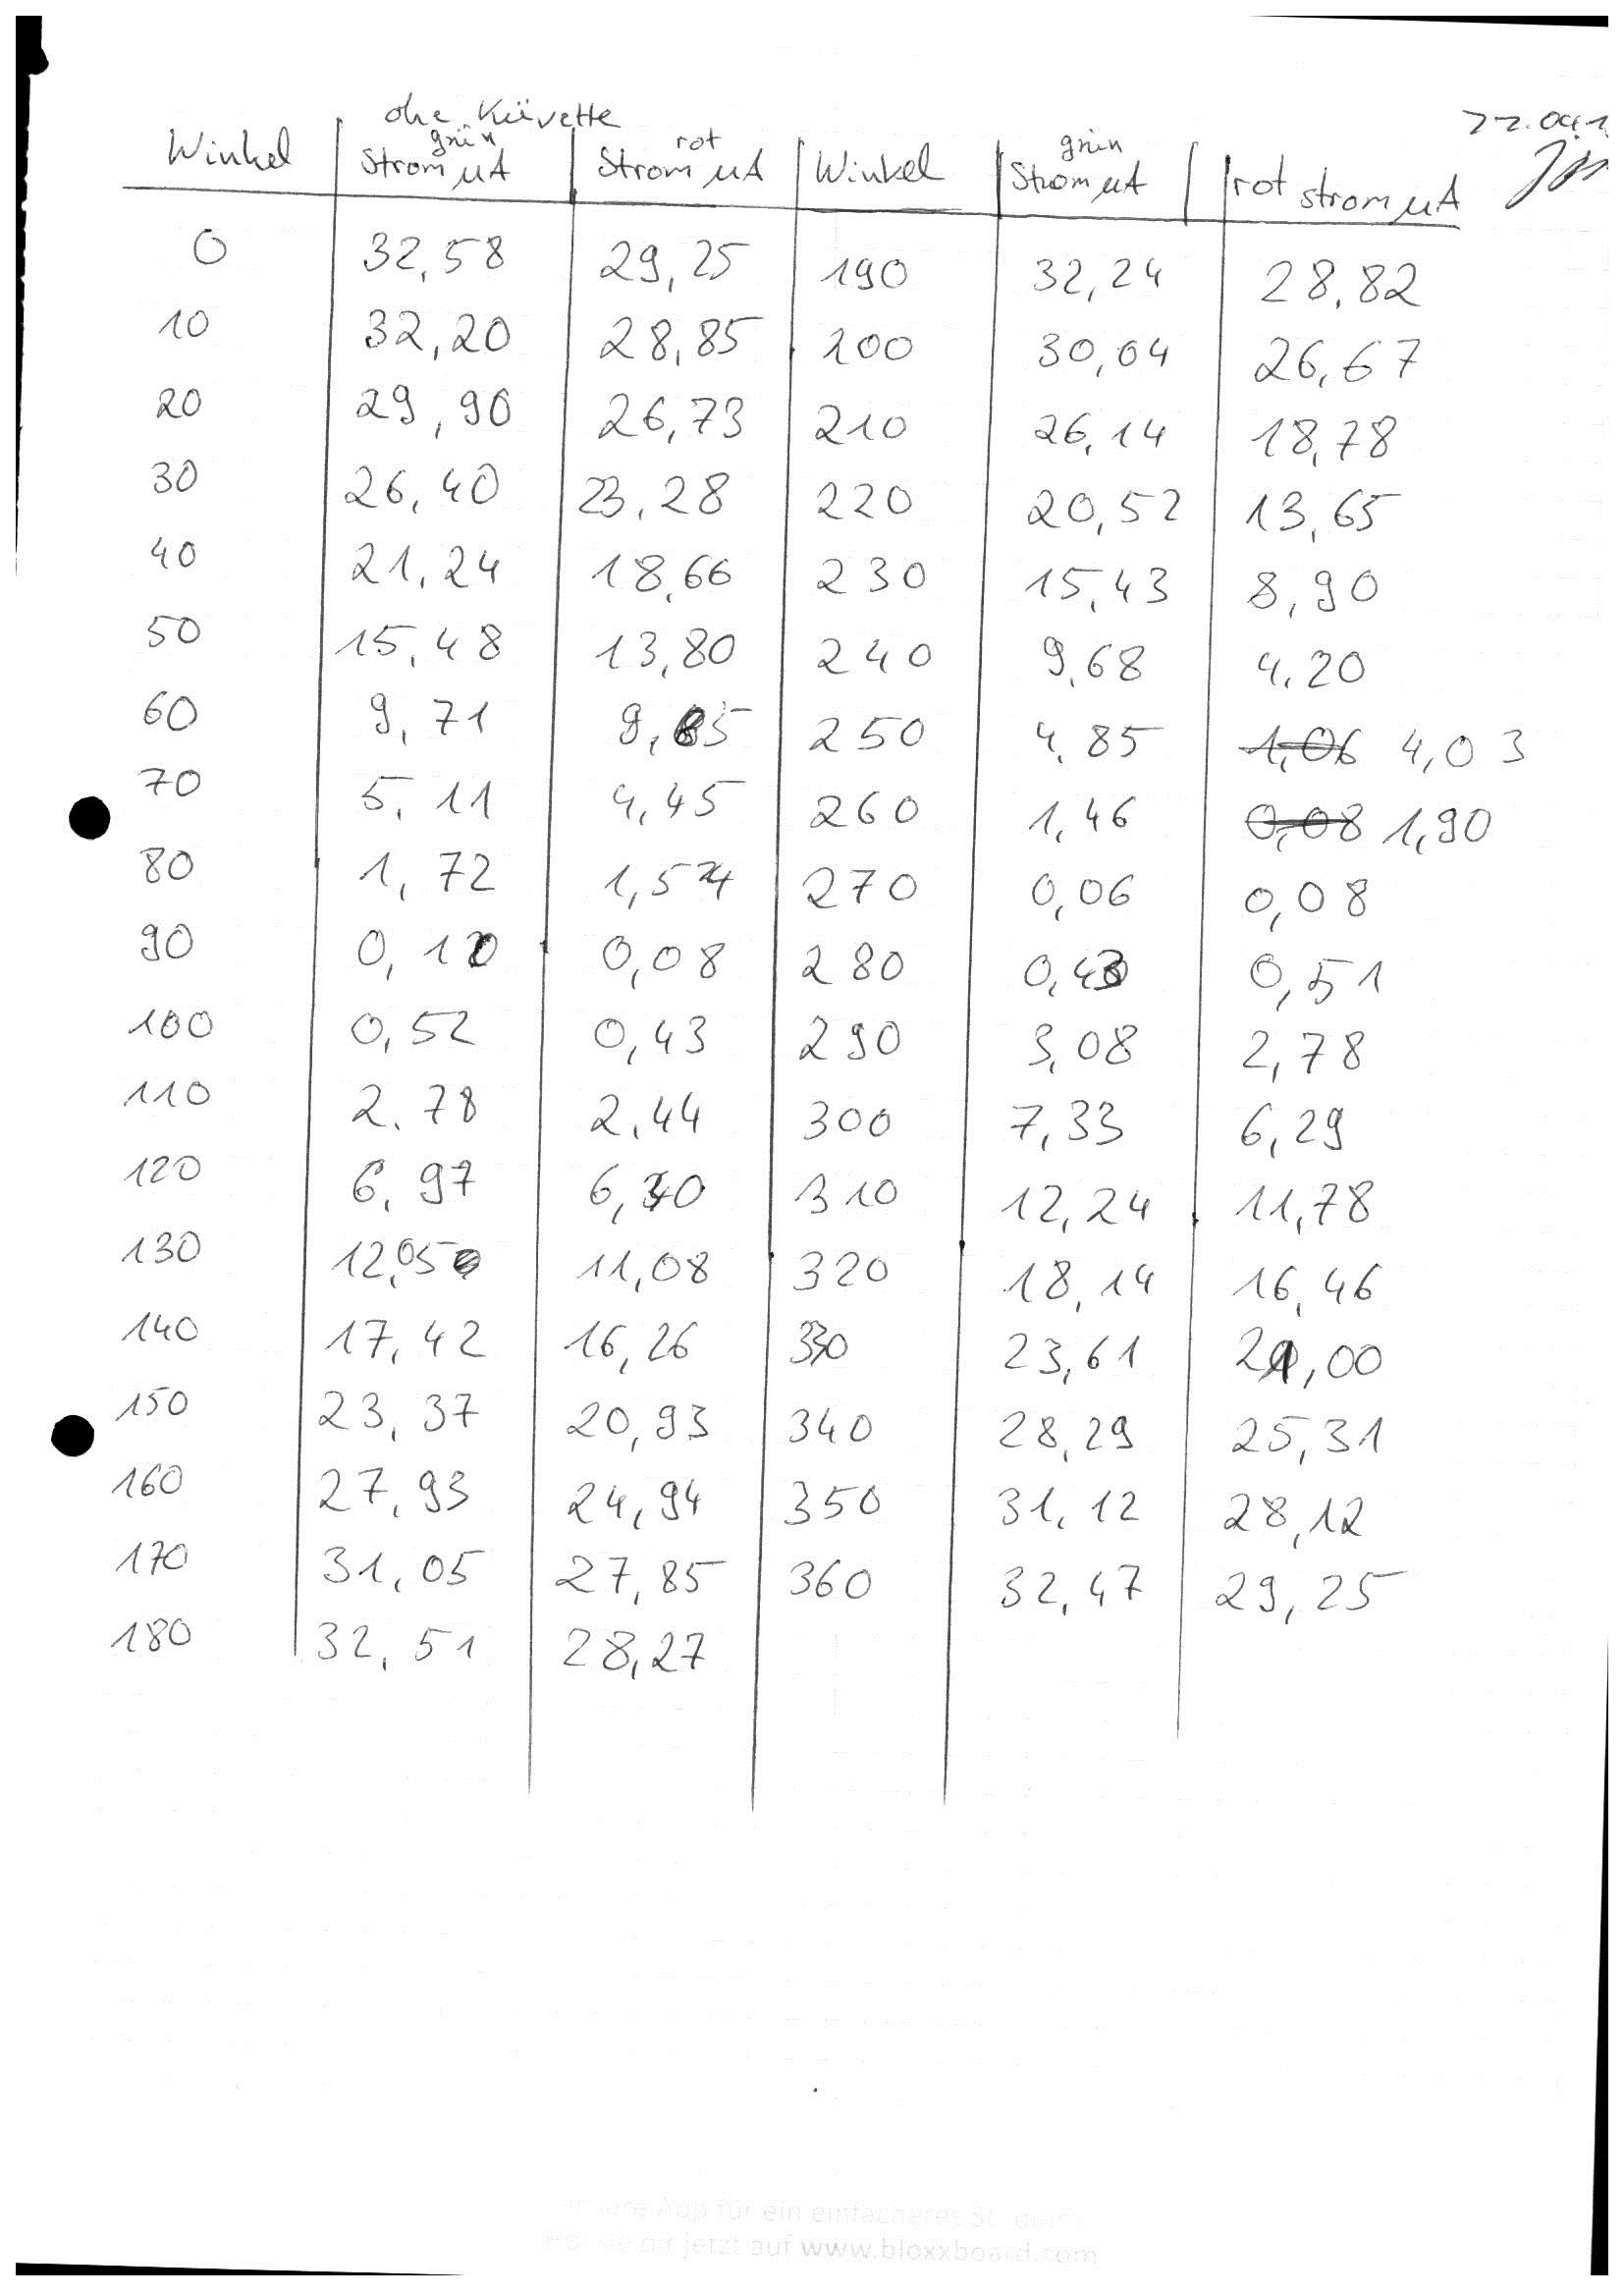
\includegraphics[scale=0.6]{Graphik/3}
        \vspace{-10pt}

\end{figure}
\begin{figure}[H]
\vspace{-17pt}
        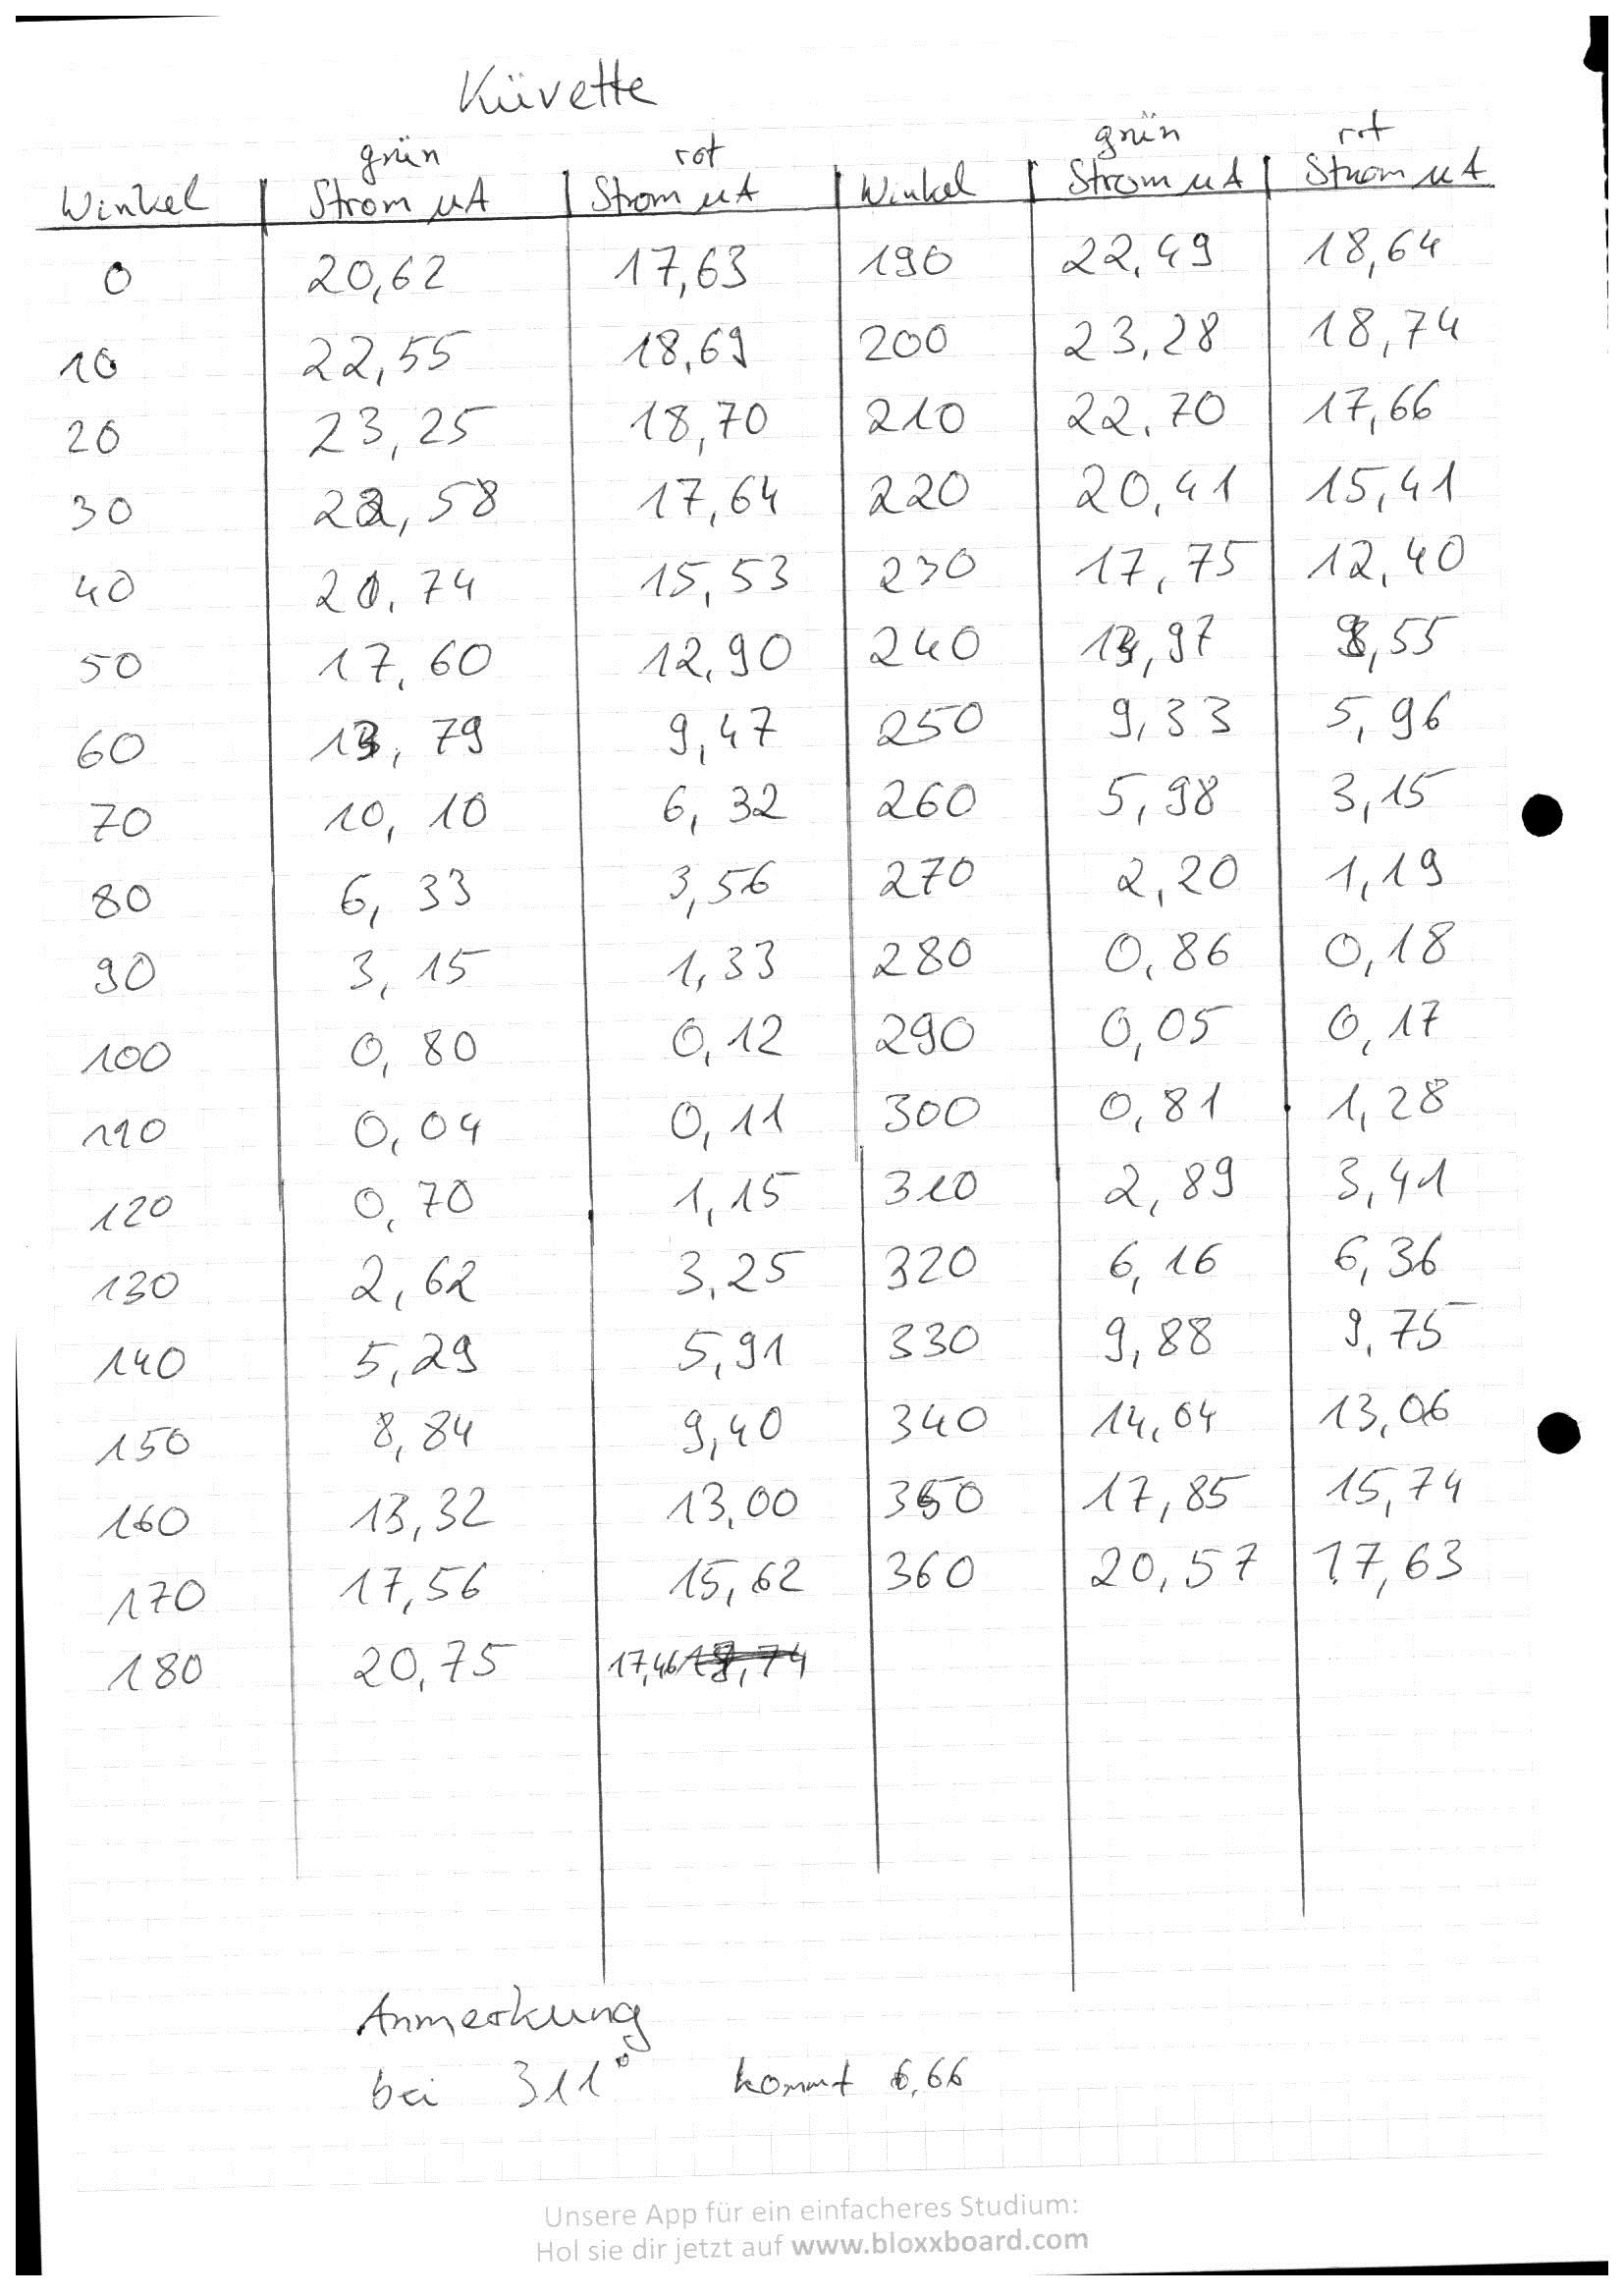
\includegraphics[scale=0.6]{Graphik/4}
        \vspace{-10pt}

\end{figure}

\end{document}
